\chapter{Physical Model and System of Equations}
    \BA{Introduction.}
    
    \BA{Room for lots of pictures here.}
    
    \BA{What physics characterize a (magnetized) neutral plasma? Quasi-neutral mix of \emph{separated} electrically-charged phases. (Check out the \href{https://en.wikipedia.org/wiki/Plasma_(physics)}{plasma Wikipedia page}.)}
    
    \BA{Will make the assumptions:
    \begin{itemize}
        \item  Only 2 phases (positive and negative) i.e.:
        \begin{itemize}
            \item  The plasma is fully ionized, i.e. neutrals (or at least the effects thereof) are negligible. I've been led to believe this is generally the case in edge plasmas (i.e. outside the divertor). (A bold assumption?)
            \item  Dust and impurities (or at least the effects thereof) are negligible. (A bold assumption?)
        \end{itemize}
        \item  Only (thermalizing) Coulomb collisions are considered- these are generally dominant over the others in a tokamak. (N.B. No fusion.)
        \item  Relativistic effects are negligible. (Is observing that the velocity scale is much smaller than $c$ sufficient justification? Imperial guy at the NEPTUNE workshop appeared to think not.)
    \end{itemize}}
    
    
    \section{Fluid Models: The \emph{High} Collisionality Limit}
    It is often the case that on the typical parameter scales of interest, the collisional terms massively dominate the kinetic Boltzmann equation. \BA{(Dimensional analysis here? Or at least some note saying that this is natural to expect from the typical \emph{very high} particle densities we encouter in daily life.)}
    
    \subsection{Single-Phase Fluids}
        When the collisional terms are dominant in the single-phase fluid Boltzmann equation (\ref{eqn:single-phase Boltzmann equation}) we find, up to leading order
        \begin{align}
            0  &\sim  \mu\nabla_{\bfv}\cdot[f(\bfv - \bfu)] + \frac{\sigma^{2}}{2}\Delta_{\bfv}[f]  \\
            f  &\sim  \frac{\rho}{m}\sqrt{\frac{m}{k_{B}T}}^{3}\exp\left(- \frac{m}{2k_{B}T}\|\bfv - \bfu\|^{2}\right)
        \end{align}
        where $\rho$, $\bfu$, $T$—functions of $\bfx$ (and $t$)—are moments characterising the conserved quantities of mass, momentum and energy:
        \begin{align}
            \rho  &=  \int fmd\bfv  \\
            \rho\bfu  &=  \int fm\bfv d\bfv  \\
            \frac{1}{2}\rho\left(\|\bfu\|^{2} + 3\frac{k_{B}T}{m}\right)  &=  \int f\frac{1}{2}m\|\bfv\|^{2}d\bfv
        \end{align}
        and, by its definition from the energy equation here, \BA{(Don't like the way that's phrased...)} $k_{B}  \approx  1.381\times10^{- 23}\rmJ\rmK^{- 1}$ is the Boltzmann constant.
    
    \subsection{Multi-Phase Fluids}
    \subsection{Tokamak Plasmas}
    \section{Coupled Fluid/Correction Models: A \emph{Low} Collisionality Concept}
    \BA{How we can re-adapt the techniques that traditionally give a fluid model when the collision operator is non-dominant to get an accurate fluid model, to apply modern techniques in fluid simulation?}
    
    \BA{Expand as a sum of a Maxwellian and some correction!}
    
    \subsubsection*{Fluid Background: A \emph{Fluid} Model}
        \BA{Ideas already well-developed!}
        
        \BA{Correction contribution not too problematic (hopefully).}
        
    \subsubsection*{Non-Maxwellian Correction: A \emph{Kinetic} Model}
        \BA{Not just kicking the problem down the road- plasma is thermalised/Maxwellian in ``most places'' for ``most physically relevant simulations'', so the correction is (compartively) small in ``most places''.}
        
        \BA{This works so nicely, because — at least in the continuous case — having the fluid model satisfied should mean that all the relevant moments of the non-Maxwellian correction should remain at 0 for all time, thus meaning we don't have to fiddle around with evaluating the moments of the correction, or particle-on-particle collisions etc. (\emph{very} parallelisable). How well this'll carry over to the discrete simulation, only time will tell.}
        
        \BA{How do we model this:
        \begin{itemize}
            \item  Lattice Boltzmann?
            \item  Some series expansion?
            \item  Particle-in-cell (PIC)?  \\
            One thing worthy of note that I'm concerned about is how a PIC model would handle different tail behaviours for very-high-energy particles. In tokamak plasmas for example, Alfvénic damping of particles with velocities above the Alfvén velocity causes particle energy distributions to have a cut-off that is $\ll  \exp\left(- {\rm const.}\|\bfv\|^2\right)$ as $\|\bfv\|  \rightarrow  \infty$ (see figure \ref{sharp cut-off energy distributions}). Salomon seems to believe this has a strong effect on the plasma behaviour, and things Wayne has said would hint in this direction too. Honestly I think the response to this is just to ensure the particles are generated with enough fidelity on the tails to capture these varying behaviours, and otherwise not worry about it, unless the people at Warwick have any better suggestions? I mean honestly, how much can I do about this? Would need to understand the theory a little better first.
        \end{itemize}}
        
        \begin{figure}[!h]
            \centering
            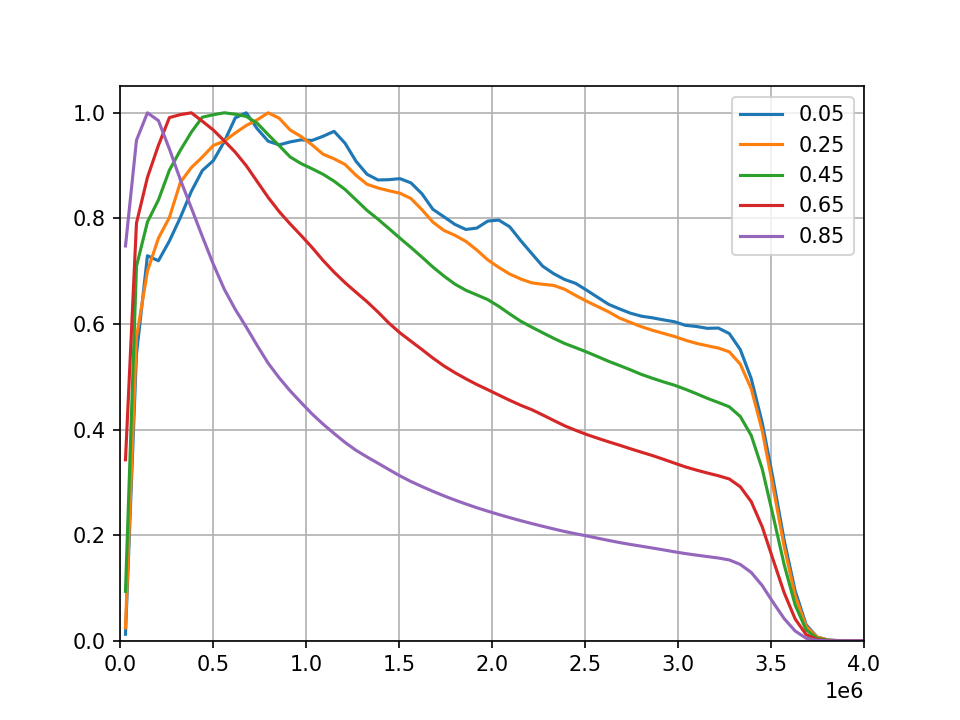
\includegraphics{paper/1 - physical model and system of equations/4 - coupled fluid correction models/images/sharp cut-off energy distributions.png}
            \caption{Experimental energy distribution function for alpha particles over different flux tubes of varying minor radius within a tokamak, showing the sharp cut-off when the energy reaches a certain threshold corresponding to the Alfvén velocity. \BA{(Since this diagram came from Tokamak Energy, I'm very wary that I probably can't use it in my final transfer thesis, but it's useful here for demonstration purposes.)}}
            \label{sharp cut-off energy distributions}
        \end{figure}
    
    
    \subsection{Single-Phase Fluids}
        \BA{Need to run some simulations this model works, testing for exclusively kinetic effects:
        \begin{itemize}
            \item  One region of fluid passing through another- this should \emph{really} highlight the effectiveness of the coupled fluid/correction model!
            \item  Kinetic fluid waves? I'm not sure those are a thing...
        \end{itemize}}
    
    
    \subsection{Multiphase Fluids}
    
    
    \subsection{Tokamak Plasmas}
        \BA{Again, need to run some simulations this model works, testing for exclusively kinetic effects:
        \begin{itemize}
            \item  Similar can do one region of fluid passing through another- would be interesting to see how this differs from the original single-phase fluid simulations.
            \item  Kinetic plasma waves. There's a \href{https://en.wikipedia.org/wiki/Waves_in_plasmas}{\emph{lot}} of these!
        \end{itemize}}
    \section{Edge Plasma Model}
    \BA{Little about the edge plasma model we're going to consider:
    \begin{itemize}
        \item  Looking for symmetric structures on a low aspect ratio?
        \item  Idk there's a lot of ways to consider this- I could very well end up doing different kinds of simulations with all different kinds of BCs in the final product, and seeing how my results match up.
    \end{itemize}}
    

    \section*{Summary}
        \BA{Summary.}